
% v2-acmsmall-sample.tex, dated March 6 2012
% This is a sample file for ACM small trim journals
%
% Compilation using 'acmsmall.cls' - version 1.3 (March 2012), Aptara Inc.
% (c) 2010 Association for Computing Machinery (ACM)
%
% Questions/Suggestions/Feedback should be addressed to => "acmtexsupport@aptaracorp.com".
% Users can also go through the FAQs available on the journal's submission webpage.
%
% Steps to compile: latex, bibtex, latex latex
%
% For tracking purposes => this is v1.3 - March 2012
\documentclass[prodmode,acmtecs]{acmsmall} % Aptara syntax
\usepackage[spanish,polish]{babel}
\usepackage[T1]{fontenc}
\usepackage{fancyvrb}
\usepackage{graphicx,hyperref}
\newcommand\cutout[1]{}


\usepackage[table]{xcolor}
\usepackage[utf8]{inputenc}
\usepackage[parfill]{parskip}
\usepackage{tabulary}
\PassOptionsToPackage{hyphens}{url}
\usepackage{hyperref}    
\usepackage[capitalize]{cleveref}


% Metadata Information
% !!! TODO: SET THESE VALUES !!!
\acmVolume{0}
\acmNumber{0}
\acmArticle{CFP}
\acmYear{0}
\acmMonth{0}

\newcounter{colstart}
\setcounter{page}{4}

\RecustomVerbatimCommand{\VerbatimInput}{VerbatimInput}%
{
%fontsize=\footnotesize,
fontfamily=\rmdefault
}


\newcommand{\UnderscoreCommands}{%\do\verbatiminput%
\do\citeNP \do\citeA \do\citeANP \do\citeN \do\shortcite%
\do\shortciteNP \do\shortciteA \do\shortciteANP \do\shortciteN%
\do\citeyear \do\citeyearNP%
}

\usepackage[strings]{underscore}



% Document starts
\begin{document}


\setcounter{colstart}{\thepage}

\acmArticle{CFP}
\title{\huge\sc SIGLOG Monthly 228}
\author{DAVID PURSER\affil{University of Warsaw, Poland}
\vspace*{-2.6cm}\begin{flushright}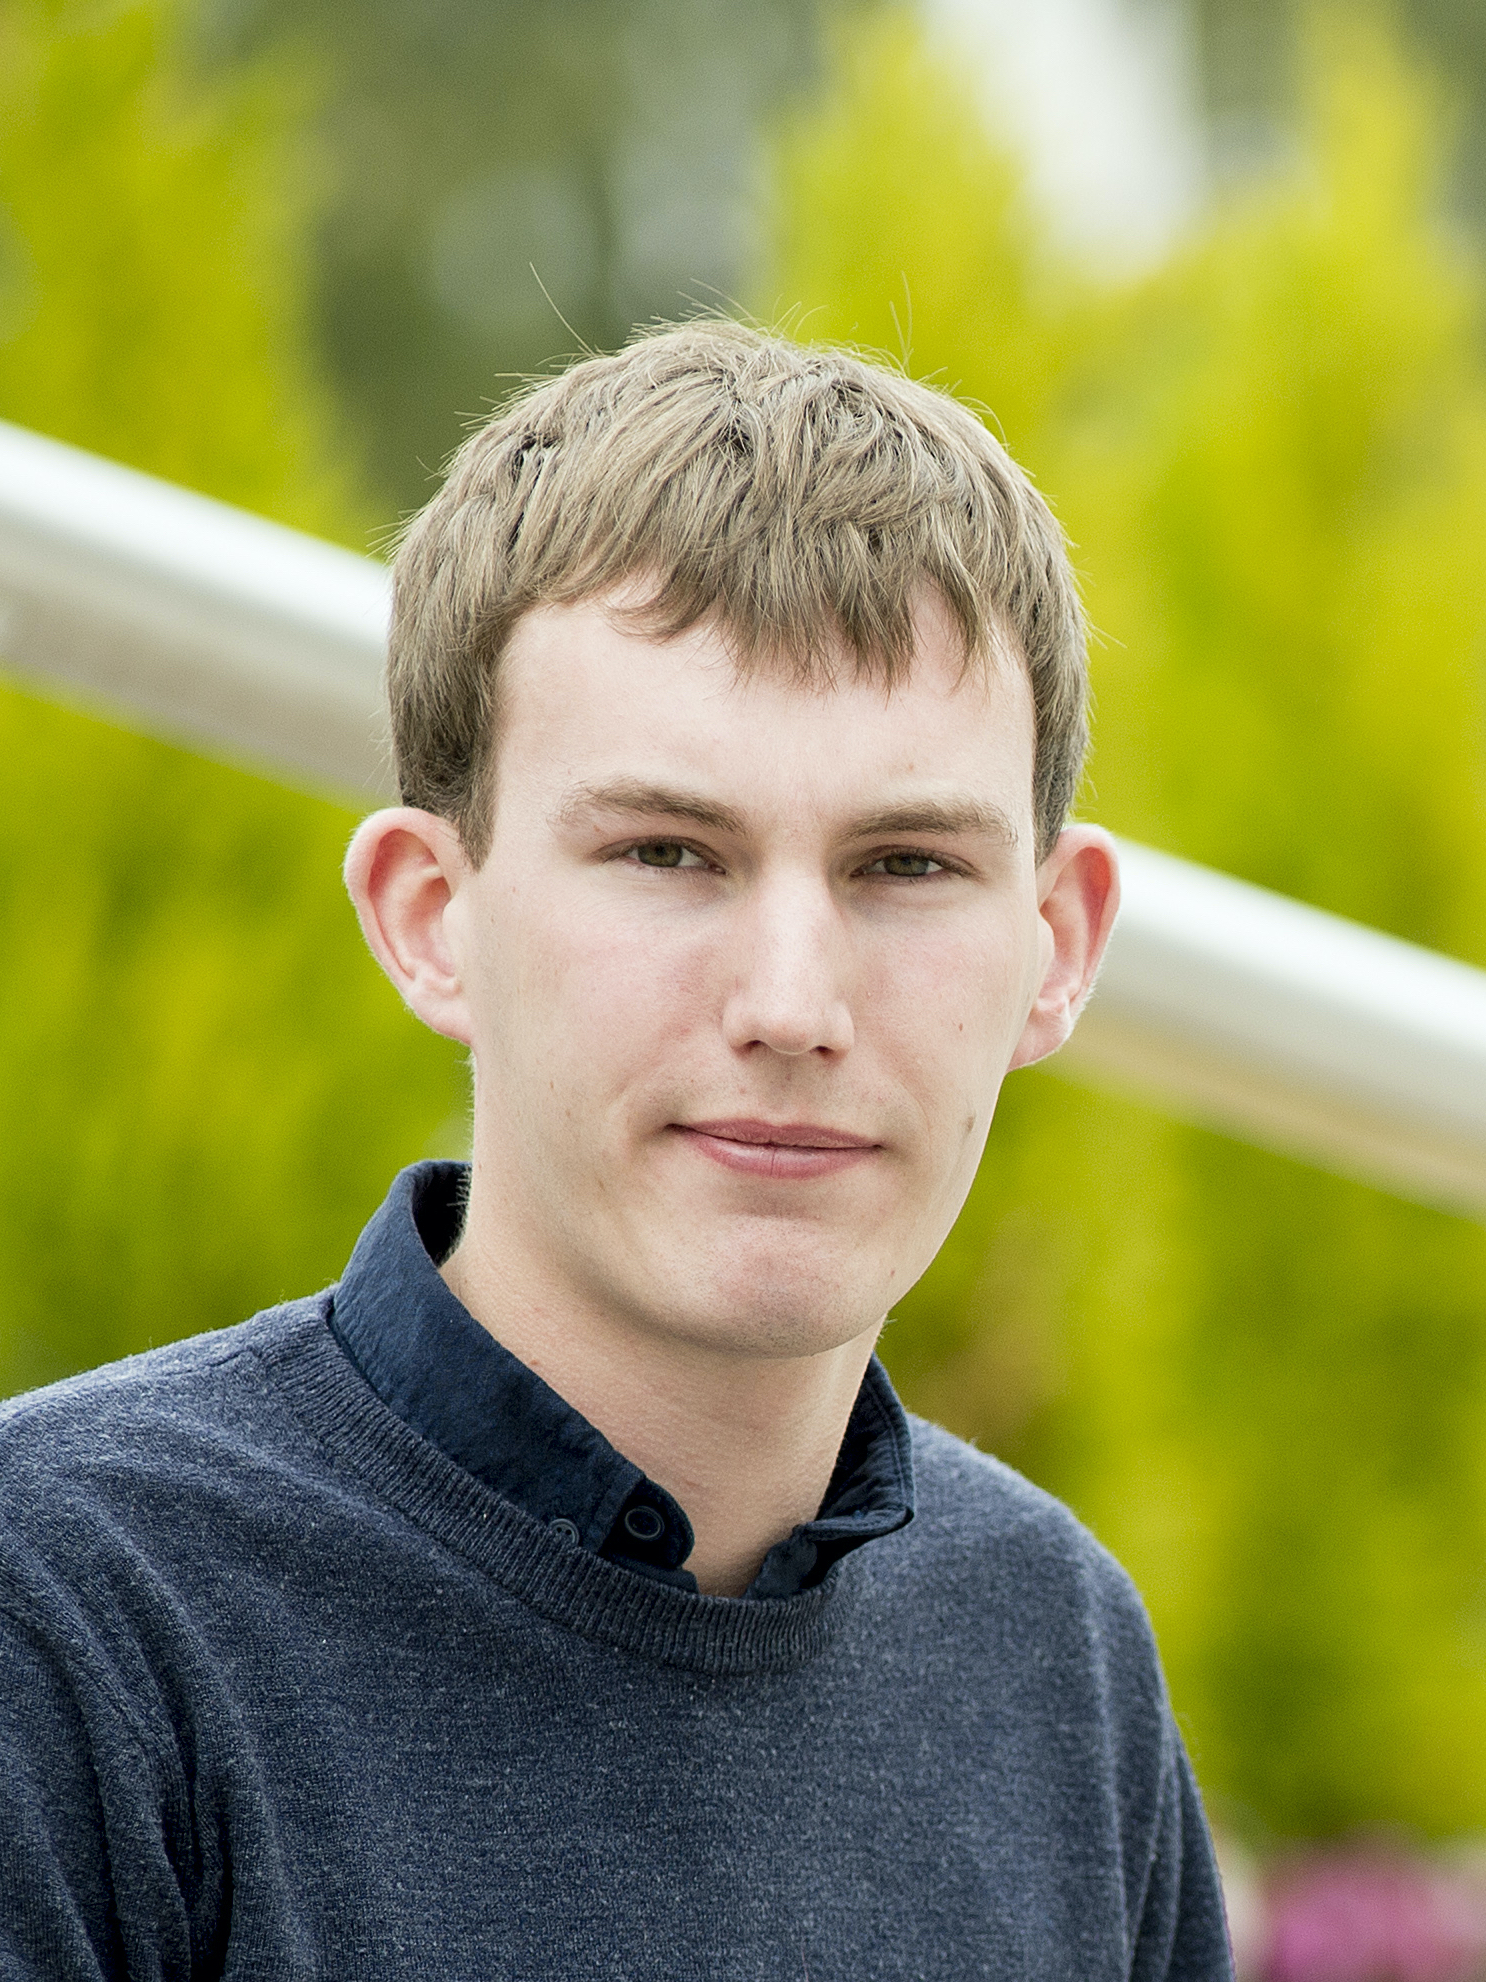
\includegraphics[width=30mm]{dp}\end{flushright}
}

\maketitlee

\href{https://lics.siglog.org/newsletters/}{Past Issues}
 - 
\href{https://lics.siglog.org/newsletters/inst.html}{How to submit an announcement}
\section{Table of Content}\begin{itemize}\item DEADLINES (\cref{deadlines}) 
 
\item SIGLOG MATTERS 
 
\begin{itemize}\item FLoC (\cref{FLoC})
\end{itemize} 
\item CALLS 
 
\begin{itemize}\item AAAI-23 (CALL FOR PAPERS) (\cref{AAAI23})
\item BEWARE (CALL FOR PAPERS) (\cref{BEWARE})
\end{itemize} 
\item JOB ANNOUNCEMENTS 
 
\begin{itemize}\item PhD Student or Postdoc Position in Alexander von Humboldt Professor group (\cref{PhDStudentorPostdocPositioninAlexandervonHumboldtProfessorgroup})
\end{itemize} 
\end{itemize}\section{Deadlines}\label{deadlines}\rowcolors{1}{white}{gray!25}\begin{tabulary}{\linewidth}{LL}AAAI-23:  & Aug 08, 2022 (Abstract), Aug 15, 2022 (Paper) \\
AiML 2022:  & Aug 10, 2022 (Registration deadline) \\
The ALP Alain Colmerauer Prolog Heritage Prize:  & Sep 02, 2022 (Deadline for nominations) \\
CPP 2023:  & Sep 14, 2022 (Abstract), Sep 21, 2022 (Paper) \\
BEWARE:  & Sep 23, 2022 (Submission deadline) \\
OVERLAY 2022:  & Sep 30, 2022 (Paper) \\
FSEN 23:  & Oct 07, 2022 (Abstract), Oct 14, 2022 (Paper) \\
PODS 2023:  & Nov 28, 2022 (Second cycle abstract), Dec 05, 2022 (Full paper) \\
\end{tabulary}
\section{FLoC: The 8th Federated Logic Conference}\label{FLoC}  \href{https://www.floc2022.org/}{https://www.floc2022.org/}\\ 
SIGLOG MATTER 

\begin{itemize}\item  Registration is still possible: \href{https://www.floc2022.org/registration}{https://www.floc2022.org/registration} 
 
\item  Reminder of the program: \href{https://easychair.org/smart-program/FLoC2022/index.html}{https://easychair.org/smart-program/FLoC2022/index.html} 
 
\end{itemize}\section{AAAI-23: Special Track on Safe and Robust AI}\label{AAAI23}  \href{https://aaai.org/Conferences/AAAI-23/safeandrobustai}{https://aaai.org/Conferences/AAAI-23/safeandrobustai} \\ 
  \href{https://aaai.org/Conferences/AAAI-23/aaai23call}{https://aaai.org/Conferences/AAAI-23/aaai23call}\\ 
CALL FOR PAPERS 

\begin{itemize}\item  We are pleased to announce that AAAI-23 will have a new special track on Safe and Robust AI, covering research on creating safe and robust AI systems, as well as using AI to create other safe and robust systems. We invite you to submit your contributions to this special track at AAAI-23. 
 
\item  AIMS AND SCOPE 
 
  This special track focuses on the theory and practice of safety and robustness in AI-based systems. AI systems are increasingly being deployed throughout society within different domains such as data science, robotics and autonomous systems, medicine, economy, and safety-critical systems. Although the widespread use of AI systems in today's world is growing, they have fundamental limitations and practical shortcomings, which can result in catastrophic failures. Specifically, many of the AI algorithms that are being implemented nowadays fail to guarantee safety and success and lack robustness in the face of uncertainties.  
 
  To ensure that AI systems are reliable, they need to be robust to disturbance, failure, and novel circumstances. Furthermore, this technology needs to offer assurance that it will reasonably avoid unsafe and irrecoverable situations. In order to push the boundaries of AI systems' reliability, this special track at AAAI-23 will focus on cutting-edge research on both the theory and practice of developing safe and robust AI systems. Specifically, the goal of this special track is to promote research that studies 1) the safety and robustness of AI systems, 2) AI algorithms that are able to analyze and guarantee their own safety and robustness, and 3) AI algorithms that can analyze the safety and robustness of other systems. For acceptance into this track, we would expect papers to have fundamental contributions to safe and robust AI, as well as applicability to the complexity and uncertainty inherent in real-world applications. 
 
  In short, the special track covers topics related to safety and robustness of AI-based systems and to using AI-based technologies to enhance the safety and robustness of themselves and other critical systems, including but not limited to:  
 
\begin{itemize}\item  Safe and Robust AI Systems
\item  Safe Learning and Control
\item  Quantification of Uncertainty and Risk
\item  Safe Decision Making Under Uncertainty and Limited Information
\item  Robustness Against Perturbations and Distribution Shifts
\item  Detection and Explanation of Anomalies and Model Misspecification
\item  Formal Methods for AI Systems
\item  On-line Verification of AI Systems
\item  Safe Human-Machine Interaction
\end{itemize} 
\item  SUBMISSION INSTRUCTIONS  
 
  Submissions to this special track will follow the regular AAAI technical paper submission procedure, but the authors need to select the Safe and Robust AI special track (SRAI). 
 
\item  IMPORTANT DATES (AoE) 
 
\rowcolors{1}{white}{gray!25}\begin{tabulary}{\linewidth}{LL}Abstract submission:  & Aug 08, 2022 \\
Paper submission:  & Aug 15, 2022 \\
\end{tabulary}
 
\end{itemize}\section{BEWARE:}\label{BEWARE}  \href{https://sites.google.com/view/beware2022/}{https://sites.google.com/view/beware2022/}\\ 
  Co-located with AIxIA 2022\\ 
  November 28 - December 2, 2022,\\ 
  University of Udine, Udine, Italy\\ 
  Joint BRIO Workshop (Bias, Risk and Opacity in AI), ME\&E-LP Workshop (Machine Ethics \& Explainability - the Role of Logic Programming), and AWARE AI Workshop (Ethics and AI, a two-way relationship)\\ 
CALL FOR PAPERS 

\begin{itemize}\item  The workshop invites submissions from computer scientists, philosophers, economists and sociologists wanting to discuss contributions ranging from the formulation of epistemic and normative principles for AI, their conceptual representation in formal models, to their development in formal design procedures and translation into computational implementations. 
 
\item  TOPICS 
 
  Topics of interest include, but are not at all limited to: 
 
\begin{itemize}\item  Conceptual and formal definitions of bias, risk and opacity in AI 
\item  Epistemological and normative principles for fair and trustworthy AI 
\item  Ethical AI and the challenges brought by AI to Ethics 
\item  Explainable AI 
\item  Uncertainty in AI 
\item  Ontological modelling of trustworthy as opposed to biased AI systems 
\item  Defining trust and its determinants for implementation in AI systems 
\item  Methods for evaluating and comparing the performances of AI systems 
\item  Approaches to verification of ethical behaviour 
\item  Logic Programming Applications in Machine Ethics 
\item  Integrating Logic Programming with methods for Machine Ethics and Explainable AI
\end{itemize} 
  Submission The workshop invites (possibly non-original) submissions of FULL PAPERS (up to 15 pages) and SHORT PAPERS (up to 5 pages). Short papers are particularly suitable to present work in progress, extended abstracts, doctoral theses, or general overviews of research projects. Note that all papers will undergo a careful peer-reviewer process and, if accepted, camera-ready versions of the papers will be published on the AIxIA subseries of CEUR proceedings (Scopus indexed). 
 
  Manuscripts must be formatted using the 1-column CEUR-ART Style. For more information, please see the CEUR website \href{http://ceur-ws.org/HOWTOSUBMIT.html}{http://ceur-ws.org/HOWTOSUBMIT.html}. Papers must be submitted through EasyChair \href{https://easychair.org/conferences/?conf=beware22}{https://easychair.org/conferences/?conf=beware22}. 
 
\item  IMPORTANT DATES  
 
\rowcolors{1}{white}{gray!25}\begin{tabulary}{\linewidth}{LL}Submission deadline:  & Sep 23, 2022 \\
Notification:  & Oct 21, 2022 \\
Camera ready:  & Nov 18, 2022 \\
\end{tabulary}
 
\item  ORGANIZATION AND PROGRAMME COMMITTEE  
 
  \href{https://sites.google.com/view/beware2022/organization-and-pc}{https://sites.google.com/view/beware2022/organization-and-pc}  
 
\end{itemize}\section{PhD Student or Postdoc Position in Alexander von Humboldt Professor group}\label{PhDStudentorPostdocPositioninAlexandervonHumboldtProfessorgroup}JOB ANNOUNCEMENT 

\begin{itemize}\item  The group of André Platzer, the Alexander von Humboldt Professor for Logic of Autonomous Dynamical Systems, in the Department of Informatics at KIT is recruiting a PhD student or postdoc (TVL E13, full-time). Our research develops the logical foundations for cyber-physical systems and practical theorem proving tools for analyzing and correctly building such systems, including the theorem prover KeYmaera X, verified runtime monitoring ModelPlex, verified compilation, and verified safe machine learning techniques. Our techniques are used to analyze the safety of autonomous cars, airplanes and collision avoidance protocols in aerospace applications, robotics, and train control. 
 
\item  REQUIREMENTS 
 
  Key requirements for successful applications: 
 
\begin{itemize}\item  Strong demonstrable commitment to research.
\item  Strong background in logic, formal methods, theorem proving, or programming language theory.
\item  Strong background in mathematics, physics, or engineering.
\item  Excellent M.Sc. degree in computer science, mathematics or related subjects.
\item  Proficiency in English, excellent speaking and writing skills.
\item  Experience in software development projects is a plus.
\end{itemize} 
  The successful candidate is able to quickly get into new research areas and will be responsible for actively engaging in novel research questions, publishing and communicating research results, advising junior students, assisting in research grants, implementation of research results in formal methods tools, and demonstrating their applicability in cyber-physical systems applications. 
 
\item  FACULTY / DIVISION: 
 
  Alexander von Humboldt Professor on Logic of Autonomous Dynamical Systems 
 
\item  INSTITUTE: 
 
  Institute of Information Security and Dependability (KASTEL) 
 
\item  STARTING DATE:  
 
  Immediately 
 
\item  CONTACT PERSON:  
 
  André Platzer \href{https://lfcps.org/pub/job-ad.html}{https://lfcps.org/pub/job-ad.html} 
 
\end{itemize}


To the \href{http://siglog.org/}{SIGLOG} or \href{https://lics.siglog.org}{LICS} website\end{document}